% Template for Cogsci submission with R Markdown

% Stuff changed from original Markdown PLOS Template
\documentclass[10pt, letterpaper]{article}

\usepackage{cogsci}
\usepackage{pslatex}
\usepackage{float}
\usepackage{caption}

% amsmath package, useful for mathematical formulas
\usepackage{amsmath}

% amssymb package, useful for mathematical symbols
\usepackage{amssymb}

% hyperref package, useful for hyperlinks
\usepackage{hyperref}

% graphicx package, useful for including eps and pdf graphics
% include graphics with the command \includegraphics
\usepackage{graphicx}

% Sweave(-like)
\usepackage{fancyvrb}
\DefineVerbatimEnvironment{Sinput}{Verbatim}{fontshape=sl}
\DefineVerbatimEnvironment{Soutput}{Verbatim}{}
\DefineVerbatimEnvironment{Scode}{Verbatim}{fontshape=sl}
\newenvironment{Schunk}{}{}
\DefineVerbatimEnvironment{Code}{Verbatim}{}
\DefineVerbatimEnvironment{CodeInput}{Verbatim}{fontshape=sl}
\DefineVerbatimEnvironment{CodeOutput}{Verbatim}{}
\newenvironment{CodeChunk}{}{}

% cite package, to clean up citations in the main text. Do not remove.
\usepackage{apacite}

% KM added 1/4/18 to allow control of blind submission
\cogscifinalcopy

\usepackage{color}

% Use doublespacing - comment out for single spacing
%\usepackage{setspace}
%\doublespacing


% % Text layout
% \topmargin 0.0cm
% \oddsidemargin 0.5cm
% \evensidemargin 0.5cm
% \textwidth 16cm
% \textheight 21cm

\title{Title TBD}


\author{Kennedy Casey \\
        University of Chicago \\
        \texttt{\normalsize{kbcasey@uchicago.edu}}
\And \textbf{Mary Elliott} \\
             University of Texas at Dallas \\
             \texttt{\normalsize{maryle18@gmail.com}}
\And \textbf{Anapaula Silva Mandujano} \\
             University of Chicago \\
             \texttt{\normalsize{anapaula@uchicago.edu}}   
\And \textbf{Kimberly Shorter} \\
             University of Chicago \\
             \texttt{\normalsize{klshorter@uchicago.edu}}
\AND \textbf{Elizabeth Mickiewicz} \\
             University of Chicago \\
             \texttt{\normalsize{lizmick9@uchicago.edu}}         
\And \textbf{Mara Duquette} \\
             University of Chicago \\
             \texttt{\normalsize{duquettemara@uchicago.edu}}
\And \textbf{Elika Bergelson} \\
             Duke University \\
             \texttt{\normalsize{elika.bergelson@duke.edu}}
\And \textbf{Marisa Casillas} \\
             University of Chicago \\
             \texttt{\normalsize{mcasillas@uchicago.edu}}}

\newlength{\cslhangindent}
\setlength{\cslhangindent}{1.5em}
\newenvironment{CSLReferences}%
  {}%
  {\par}

\begin{document}

\maketitle

\begin{abstract}


\textbf{Keywords:}

\end{abstract}

\hypertarget{introduction}{%
\section{Introduction}\label{introduction}}

The artifacts of everyday life reflect our routines, aspirations,
relationships, and more. In particular, the objects that we regularly
pick up and handle---a coffee cup, a laptop, a baby bottle---offer a
window into the physical, social, and cultural contexts that shape our
understanding of the world. In this paper, we take a glimpse into
everyday life at its beginnings by exploring object handling at home by
children from early infancy until age four. We contextualize our study
with respect to the effects of object-centric interaction on word
learning, though we note that different analyses of these same data
could shed new light on other types of social learning as well as motor
development (see Herzberg, Fletcher, Schatz, \& Tamis-LeMonda, 2021 on
the latter point).

\hypertarget{object-handling-and-word-learning}{%
\subsection{Object handling and word
learning}\label{object-handling-and-word-learning}}

For young learners, objects and their associated activities form a
critical source of input for social learning, including the ways in
which children are exposed to language about those objects. Hands (and
what they are handling) can be reliable indicators of what someone is
doing and talking about during object play, facilitating children's
ability to map word forms onto their meanings in and across real-time
interaction (e.g., Yu \& Smith, 2013; Yurovsky, Smith, \& Yu, 2013).
Present, attended-to objects also influence the babble of children who
have acquired stable consonants (Laing \& Bergelson, 2020). Further,
caregivers' tendency to use nouns referring to objects in the
here-and-now positively predicts their children's early word
comprehension (Bergelson \& Aslin, 2017).

How frequently do children engage in object-centric interactions?
Hands---others' and their own---are in good supply in young children's
view of the world, especially after early infancy (Fausey, Jayaraman, \&
Smith, 2016; Jayaraman, Fausey, \& Smith, 2017; Long, Kachergis,
Agrawal, \& Frank, 2020), topping out at visible presence
\textasciitilde30\% of the time. Infants own object handling is also
relatively frequent: Herzberg and colleagues (2021) find that US infants
handle objects \textasciitilde60\% of the time during at-home play, Yu
and colleagues (2013) find \textasciitilde70\% when including joint
handling with adults in US in-lab object play, and Casillas \& Elliott
(2021) find \textasciitilde15 and \textasciitilde17\% object handling in
daylong photo streams in a Papuan and a Mayan community, respectively.
Note, however, that \emph{labeling} of object-relevant features (e.g.,
its name and associated concepts) is the critical second ingredient
relevant for word learning, which may only occur during a small subset
of total object handling time. Additionally, the likelihood of talk
about objects that are being handled in the here and now---a flagship
feature of contingent caregiver talk (e.g., McGillion et al.,
2013)---fluctuates across high and low activity periods of interaction
(Bergelson, Amatuni, Dailey, Koorathota, \& Tor, 2019).

Overall, while prior work makes a strong case for the impact of
children's object-centric interactions on their word learning, the
findings: (a) are limited to a culturally narrow sample of populations,
(b) have tended to rely on short recordings that limit the scope of
object-centered interactions analyzed, and (c) have rarely examined in
detail the distributions of individual objects children typically
interact with at home Herzberg, Fletcher, Schatz, \& Tamis-LeMonda
(2021).

\hypertarget{object-handling-across-age-and-culture}{%
\subsection{Object handling across age and
culture}\label{object-handling-across-age-and-culture}}

Children's object handling input changes enormously across the first few
years due to both maturational constraints and culture-specific
caregiving practices. In early infancy, children have little ability to
hold things or to control their posture, primarily experiencing objects
through what others bring near to them (faces may make up a much greater
proportion of their social input at this point; Fausey, Jayaraman, \&
Smith (2016); Jayaraman, Fausey, \& Smith (2017), but see Long,
Kachergis, Agrawal, \& Frank (2020)). However, later gains in manual
dexterity and gross motor skill (e.g., sitting, crawling, walking)
increasingly widen their ability to seek, reach, and grab a diversity of
objects in their environment and give them greater control over what
they handle, how they elicit social information relating to that object,
and for how long (Adolph, Karasik, \& Tamis-LeMonda, 2010; Gaskins,
2000; Herzberg, Fletcher, Schatz, \& Tamis-LeMonda, 2021; Kretch,
Franchak, \& Adolph, 2014; Sanchez, Long, Kraus, \& Frank, 2018).

Early access to objects is also shaped by culture-specific practices for
carrying children, keeping them safe and warm, and scaffolding the
development of locally valued capacities (e.g., word learning in many US
families, walking in Kenyan Kipsigis families, Super (1976), see Adolph,
Karasik, \& Tamis-LeMonda (2010) for an overview). The array of objects
available to children will also vary in type and prevalence
crossculturally, including: (a) objects spread via globalization (e.g.,
plastic bags), (b) objects that have a basic functional role that has
arisen similarly across many groups (e.g., spoon-like things for
eating), and (c) objects are specific to people and places (e.g., the
gourd and bombilla for drinking mate in much of South America, stemming
from Indigenous Guaraní and Tupí tradition). Take, for example,
middle-class US family homes, which have been noted for their large
quantities of possessions (``clutter''), much of which is designed
specifically for children (e.g., toys and books Arnold, Graesch, Ochs,
\& Ragazzini (2012)). We might infer, based on this distribution, that
much of what children do and talk about at home is tailored to what
particularly interests them. And thus the children's worlds, in this
sense, look very different from their caregivers'. Recent work by
Herzberg and colleagues (2021) underscores this point with infancy data;
13--23-month-olds spent nearly 70\% of their time in object play with
toys or a mix of toys and non-toys, with \textasciitilde100\% of infants
playing with children's books and stuffed animals and a total of 32 toy
types appearing in \(\ge\) 25\% of infants' play. Non-toy play was also
common, but still appeared to predominantly include infant-specific
objects (e.g., sippy cups, baby spoons, high chairs, pacifiers). We
would expect many of these items to be rare in other parts of the world,
with much greater overlap between objects for infants and objects for
adults (e.g., Karasik, Schneider, Kuchirko, \& Tamis-LeMonda (2018,
June)).

\hypertarget{the-current-study}{%
\subsection{The current study}\label{the-current-study}}

\hypertarget{method}{%
\section{Method}\label{method}}

\hypertarget{corpus}{%
\subsection{Corpus}\label{corpus}}

We analyze daylong photo streams from child-worn cameras in two rural,
small-scale subsistence farming communities: Rossel Papuan and Tseltal
Mayan. While these horticulturalist communities are comparable,
differences in the organization of daily life as well as the
availability of certain types of objects (e.g., synthetic materials
after market integration for the Tseltal context but not Rossel) allow
for cross-cultural comparison. Daylong photo streams consist of images
captured every 15 (Rossel) to 30 (Tseltal) seconds over the course of 8
(Rossel) to 9 (Tseltal) hours at home. Children wore a recording vest
equipped with a camera (Narrative Clip 1) and miniature fisheye lens
(Photojojo Super Fisheye) that provided a 180\(\text{\textdegree}\) view
of the environment. For younger infants who were not yet walking, the
camera was instead worn by the primary caregiver. Here, we analyze the
subset of photos known to feature child object handling based on prior
work with the same data sets (Casillas \& Elliott, 2021).

The present data include images from 56 children (Rossel: 27, Tseltal:
27) ranging in age from 0 to 48 months
(\emph{M}\textsubscript{\emph{Rossel}} = 21.5,
\emph{M}\textsubscript{\emph{Tseltal}} = 22.7). For each child, a range
of 1 to 653 photos were annotated (\emph{M}\textsubscript{\emph{Rossel}}
= 21.5, \emph{M}\textsubscript{\emph{Tseltal}} = 22.7).

\hypertarget{manual-annotation}{%
\subsection{Manual annotation}\label{manual-annotation}}

We annotated photos with IMCO (version 2;
\url{https://github.com/kennedycasey/ImCo2}), an open-source program
adapted for efficient coding of photo streams . Annotators provided
labels for the handled object(s) present in each photo and selected
among predefined categories to characterize each type of object in the
image. Categories included food, tools, toys, immovable objects, natural
objects, and miscellaneous synthetic objects (see Table
\ref{tab:top-objects} for example objects from each category).

\hypertarget{reliability}{%
\subsection{Reliability}\label{reliability}}

XX\% of photo streams were double coded. Reliability annotations were
equally spread across sites and ages. At the category level, annotators
agreed on XX.X\% of decisions (Rossel: XX.X\%, Tseltal: XX.X\%). At the
object label level, annotators agreed on XX.X\% of decisions (Rossel:
XX.X\%). Additionally, to avoid unnecessary data loss, all excluded
photos were checked by at least one other annotator and re-included for
analysis if objects were identifiable.

\begin{table}[!ht]
\centering
\scalebox{0.8}{
\begin{tabular}{lll}
  \hline
Object Category & Rossel & Tseltal \\ 
  \hline
Synthetic & rope, shirt, plastic bottle & shirt, chair, pants \\ 
  Food & coconut, betelnut, tuber & guava, tortilla, apple \\ 
  Tool & knife, bowl, spoon & bowl, cup, bottle \\ 
  Toy & ball, book, plastic toy & book, toy truck, baby doll \\ 
  Natural & stick, rock, leaf & stick, leaf, tree \\ 
  Immovable & veranda, ladder, railing & door, fence, table \\ 
   \hline
\end{tabular}
}
\caption{Objects handled by the most children across categories and sites.} 
\label{tab:top-objects}
\end{table}

\hypertarget{results}{%
\section{Results}\label{results}}

\hypertarget{overall-frequency-statistics}{%
\subsection{Overall frequency
statistics}\label{overall-frequency-statistics}}

Children handled an average of 21.16 unique objects per day (median =
20, \emph{SD} = 15.2, range = 1--59), with no significant differences
across sites (\emph{M}\textsubscript{\emph{Rossel}} = 18.93,
\emph{M}\textsubscript{\emph{Tseltal}} = 23.24, \emph{W} = 350, \emph{p}
= 0.501). Only 20.83\% of objects were present in both communities, but
several shared objects were among the most frequently handled by
children in both sites. In fact, among the top 25 most common objects,
11 were shared across sites.

The frequency of object categories was similarly divided across sites
(Figure 1A). The top objects for each category are shown in Table 1.
Children primarily handled miscellaneous synthetic objects (e.g., rope,
guitar, shirt, etc.; \emph{M}\textsubscript{\emph{Rossel}} = 32.01\% of
handling, \emph{M}\textsubscript{\emph{Tseltal}} = 37.5\%) and food
(\emph{M}\textsubscript{\emph{Rossel}} = 28.58\%,
\emph{M}\textsubscript{\emph{Tseltal}} = 36.21\%). For 45 of 56
children, the top category was either synthetic objects or food.
Two-tailed Wilcoxon tests revealed only one significant category-level
difference between sites: children's handling of large or immovable
objects (e.g., veranda, ladder, railing, etc.), where Rossel children
handled these objects more frequently than Tseltal children
(\emph{M}\textsubscript{\emph{Rossel}} = 7.73\%,
\emph{M}\textsubscript{\emph{Tseltal}} = 3.31\%, adjusted \emph{p} =
0.038, \emph{p}s for all other categories \textgreater{} 0.05), but
these objects were still the least frequently handled in both sites.

During any given hour, children handled 5.26 objects from 2.79 different
categories, on average (median = 4.5 objects, \emph{SD} = 3.92, range =
1--18). A linear mixed-effects model with fixed effects of site, each of
6 object categories, and their interaction showed a significant main
effect of the synthetic object category (\(\beta\) = 0.52, \emph{SE} =
0.2, \emph{t} = 2.59, \emph{p} = 0.01) as well as an interaction between
site and the synthetic object category (\(\beta\) = 1.11, \emph{SE} =
0.29, \emph{t} = 3.88, \emph{p} = \textless{} 0.001) such that children
handled more unique synthetic objects per hour than any other object
category, and this effect was stronger for Tseltal children than for
Rossel children (\emph{p}s \textgreater{} 0.05 for all other main
effects and interaction terms; Figure 1B).

\begin{CodeChunk}
\begin{figure}[!ht]

{\centering 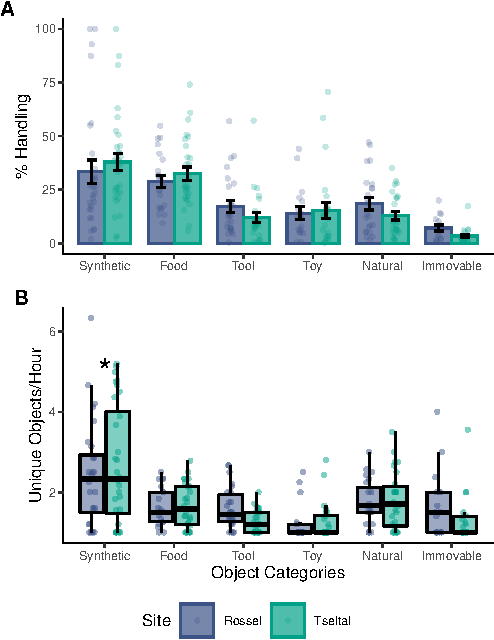
\includegraphics{figs/overall-stats-fig-1} 

}

\caption[(A) Overall frequency of handling by object category]{(A) Overall frequency of handling by object category. Points reflect percentages for individual children. (B) Count of unique objects handled per hour by object category. Points reflect means for individual children across all hours of recording.}\label{fig:overall-stats-fig}
\end{figure}
\end{CodeChunk}

\hypertarget{time-of-day-effects}{%
\subsection{Time of day effects}\label{time-of-day-effects}}

Children's overall rate of object handling was largely consistent across
the day. The number of unique handled objects per hour was not linearly
related to time of day (\(\beta\) = -0.02, \emph{SE} = 0.11, \emph{t} =
-0.16, \emph{p} = 0.874), and there was no two-way interaction between
time of day and site (\(\beta\) = 0.01, \emph{SE} = 0.14, \emph{t} =
0.1, \emph{p} = 0.923).

However, we did find differences in children's rates of holding for
specific object categories across the day. We ran individual linear
mixed-effects models, which included fixed effects of site, hour of the
day, and their interaction, for each of 6 categories. Synthetic objects
were marginally more common during the afternoon hours (\(\beta\) =
0.02, \emph{SE} = 0.01, \emph{t} = 1.71, \emph{p} = 0.09), and food
items were handled with significantly greater frequency during the
morning hours (\(\beta\) = -0.03, \emph{SE} = 0.01, \emph{t} = -2.76,
\emph{p} = 0.006; Figure 2). No other main effects or two-way
interactions reached statistical significance (all \emph{p}s
\textgreater{} 0.05).

\begin{CodeChunk}
\begin{figure}[!ht]

{\centering 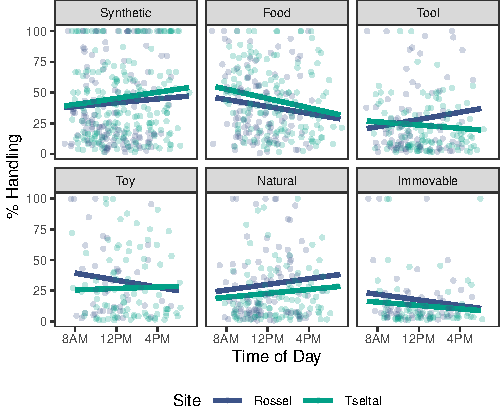
\includegraphics{figs/tod-effects-fig-1} 

}

\caption[Frequency of handling by object category across different times of day]{Frequency of handling by object category across different times of day. Individual points show raw percentages for each child, and lines reflect model-predicted percentages.}\label{fig:tod-effects-fig}
\end{figure}
\end{CodeChunk}

\hypertarget{age-effects}{%
\subsection{Age effects}\label{age-effects}}

Children's overall rate of object handling increased marginally with age
(Figure 3A). That is, older children handled more unique objects per
hour (\(\beta\) = 0.07, \emph{SE} = 0.03, \emph{t} = 1.99, \emph{p} =
0.05). Additionally, with increasing age, children handled more objects
from different categories per hour (\(\beta\) = 0.03, \emph{SE} = 0.01,
\emph{t} = 2.6, \emph{p} = 0.011). These effects were consistent across
sites; we found no main effects of site or interactions between site and
age (all \emph{p}s \textgreater{} 0.05).

\begin{CodeChunk}
\begin{figure}[!ht]

{\centering 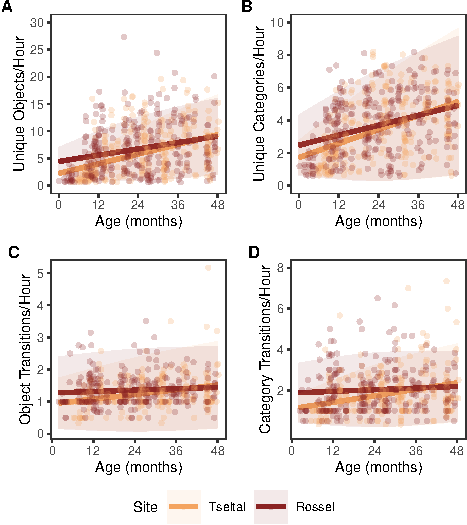
\includegraphics{figs/age-effects-fig-1} 

}

\caption[(A) Unique objects and (B) object categories handled per hour as a function of age]{(A) Unique objects and (B) object categories handled per hour as a function of age. Points reflect raw hourly counts for each child, and lines reflect model predictions with shaded standard error regions.}\label{fig:age-effects-fig}
\end{figure}
\end{CodeChunk}

\hypertarget{discussion}{%
\section{Discussion}\label{discussion}}

\hypertarget{references}{%
\section{References}\label{references}}

\setlength{\parindent}{-0.1in} 
\setlength{\leftskip}{0.125in}

\noindent

\hypertarget{refs}{}
\begin{CSLReferences}{1}{0}
\leavevmode\hypertarget{ref-adolph2010motor}{}%
Adolph, K. E., Karasik, L. B., \& Tamis-LeMonda, C. S. (2010). Motor
skill. In M. H. Bornstein (Ed.), \emph{Handbook of cultural
developmental science} (pp. 61--88). Psychology Press: New York, NY.

\leavevmode\hypertarget{ref-arnold2012life}{}%
Arnold, J. E., Graesch, A. P., Ochs, E., \& Ragazzini, E. (2012).
\emph{Life at home in the twenty-first century: 32 families open their
doors}. ISD LLC.

\leavevmode\hypertarget{ref-bergelson2019day}{}%
Bergelson, E., Amatuni, A., Dailey, S., Koorathota, S., \& Tor, S.
(2019). Day by day, hour by hour: Naturalistic language input to
infants. \emph{Developmental Science}, \emph{22}(1), e12715.

\leavevmode\hypertarget{ref-bergelson2017nature}{}%
Bergelson, E., \& Aslin, R. N. (2017). Nature and origins of the lexicon
in 6-mo-olds. \emph{Proceedings of the National Academy of Sciences},
\emph{114}(49), 12916--12921.

\leavevmode\hypertarget{ref-casillasURdaylong}{}%
Casillas, M., \& Elliott, M. (2021). Cross-cultural differences in
children's object handling at home. PsyArXiv.
http://doi.org/\href{https://doi.org/10.31234/osf.io/43db8}{10.31234/osf.io/43db8}

\leavevmode\hypertarget{ref-fausey2016faces}{}%
Fausey, C. M., Jayaraman, S., \& Smith, L. B. (2016). From faces to
hands: Changing visual input in the first two years. \emph{Cognition},
\emph{152}, 101--107.

\leavevmode\hypertarget{ref-gaskins2000childrens}{}%
Gaskins, S. (2000). Children's daily activities in a {M}ayan village: A
culturally grounded description. \emph{Cross-Cultural Research},
\emph{34}(4), 375--389.

\leavevmode\hypertarget{ref-herzberg2021exuberant}{}%
Herzberg, O., Fletcher, K. K., Schatz, J. L., \& Tamis-LeMonda, C. S.
(2021). Infant exuberant object play at home: Immense amounts of
time-distributed, variable practice. \emph{Child Development},
\emph{XX}, 1--15.

\leavevmode\hypertarget{ref-jayaraman2017faces}{}%
Jayaraman, S., Fausey, C. M., \& Smith, L. B. (2017). Why are faces
denser in the visual experiences of younger than older infants?
\emph{Developmental Psychology}, \emph{53}(1), 38.

\leavevmode\hypertarget{ref-karasik2018not}{}%
Karasik, L. B., Schneider, J., Kuchirko, Y. A., \& Tamis-LeMonda, C. S.
(2018, June2018, June). Not so {WEIRD} object play in {T}ajikistan.
Presentation to the International Conference on Infant Studies,
Philadelphia, PA.
http://doi.org/\href{https://doi.org/10.31234/osf.io/43db8}{10.31234/osf.io/43db8}

\leavevmode\hypertarget{ref-kretch2014crawling}{}%
Kretch, K. S., Franchak, J. M., \& Adolph, K. E. (2014). Crawling and
walking infants see the world differently. \emph{Child Development},
\emph{85}(4), 1503--1518.

\leavevmode\hypertarget{ref-laing2020babble}{}%
Laing, C., \& Bergelson, E. (2020). From babble to words: Infants' early
productions match words and objects in their environment.
\emph{Cognitive Psychology}, \emph{122}, 101308.

\leavevmode\hypertarget{ref-long2020detecting}{}%
Long, B., Kachergis, G., Agrawal, K., \& Frank, M. C. (2020).
\emph{Detecting social information in a dense database of infants'
natural visual experience}.

\leavevmode\hypertarget{ref-mcgillion2013supporting}{}%
McGillion, M. L., Herbert, J. S., Pine, J. M., Keren-Portnoy, T.,
Vihman, M. M., \& Matthews, D. E. (2013). Supporting early vocabulary
development: What sort of responsiveness matters? \emph{IEEE
Transactions on Autonomous Mental Development}, \emph{5}(3), 240--248.

\leavevmode\hypertarget{ref-sanchez2018detecting}{}%
Sanchez, A., Long, B., Kraus, A. M., \& Frank, M. C. (2018). Postural
developments modulate children's visual access to social information. In
\emph{Proceedings of the 40th annual conference of the cognitive science
society} (pp. 2412--2417).

\leavevmode\hypertarget{ref-super1976environmental}{}%
Super, C. M. (1976). Environmental effects on motor development: The
case of {`{A}frican infant precocity.'} \emph{Developmental Medicine \&
Child Neurology}, \emph{18}(5), 561--567.

\leavevmode\hypertarget{ref-yu2013joint}{}%
Yu, C., \& Smith, L. B. (2013). Joint attention without gaze following:
Human infants and their parents coordinate visual attention to objects
through eye-hand coordination. \emph{PloS One}, \emph{8}(11), e79659.

\leavevmode\hypertarget{ref-yurovsky2013statistical}{}%
Yurovsky, D., Smith, L. B., \& Yu, C. (2013). Statistical word learning
at scale: The baby's view is better. \emph{Developmental Science},
\emph{16}(6), 959--966.

\end{CSLReferences}

\bibliographystyle{apacite}


\end{document}
